\PassOptionsToPackage{table}{xcolor}

\documentclass[sigconf%
,natbib=true%
]{acmart}

\AtBeginDocument{%
  \providecommand\BibTeX{{%
    \normalfont B\kern-0.5em{\scshape i\kern-0.25em b}\kern-0.8em\TeX}}}

\copyrightyear{2021}
\acmYear{2021}
\setcopyright{rightsretained}
\acmConference[VINCI '21]{The 14th International Symposium on Visual Information Communication and Interaction}{September 6--8, 2021}{Potsdam, Germany}
\acmBooktitle{The 14th International Symposium on Visual Information Communication and Interaction (VINCI '21), September 6--8, 2021, Potsdam, Germany}\acmDOI{10.1145/3481549.3481573}
\acmISBN{978-1-4503-8647-0/21/09}

\acmSubmissionID{32}

\usepackage[utf8]{inputenc}
\usepackage{csquotes}
\usepackage{calc}

\usepackage{tikz}
\usetikzlibrary{calc,positioning,spy}

\begin{document}

\title[Software Galaxies]{Software Galaxies: Displaying Coding Activities\\using a Galaxy Metaphor}

\author{Daniel Atzberger}
\affiliation{%
  \institution{Hasso Plattner Institute, Digital Engineering Faculty,}
  \country{University of Potsdam, Germany}
}
\author{Willy Scheibel}
\orcid{0000-0002-7885-9857}
\affiliation{%
  \institution{Hasso Plattner Institute, Digital Engineering Faculty,}
  \country{University of Potsdam, Germany}
}
\author{Daniel Limberger}
\orcid{0000-0002-9111-4809}
\affiliation{%
  \institution{Hasso Plattner Institute, Digital Engineering Faculty,}
  \country{University of Potsdam, Germany}
}
\author{J{\"u}rgen D{\"o}llner}
\affiliation{%
  \institution{Hasso Plattner Institute, Digital Engineering Faculty,}
  \country{University of Potsdam, Germany}
}

\renewcommand{\shortauthors}{D.~Atzberger, W.~Scheibel, D.~Limberger, J.~D{\"o}llner}

\begin{abstract}
    Software visualization uses metaphors to depict software system and software development data that usually has no inherent gestalt.
    The choice of a fitting metaphor for visual display is researched broadly, but deriving a layout based on similarity is still challenging.
    We present a novel approach to 3D software visualization called \emph{Software Galaxy}.
    Our layout is based on applying Latent Dirichlet Allocation on source code documents.
    We utilize a metaphor inspired from astronomy for depicting software metrics for single documents and clusters of documents.
    Our first experiments indicate that a 3D visualization capturing semantic relatedness can be beneficial for standard program comprehension tasks.
\end{abstract}

\begin{CCSXML}
	<ccs2012>
	<concept>
	<concept_id>10003120.10003145.10003146.10010889</concept_id>
	<concept_desc>Human-centered computing~Treemaps</concept_desc>
	<concept_significance>500</concept_significance>
	</concept>
	<concept>
	<concept_id>10003120.10003145.10003147.10010923</concept_id>
	<concept_desc>Human-centered computing~Information visualization</concept_desc>
	<concept_significance>300</concept_significance>
	</concept>
	</ccs2012>
\end{CCSXML}

\ccsdesc[500]{Human-centered computing~Visual Analytics}

\keywords{Software Visualization, Visualization Metaphor, Topic Modeling}

 \begin{teaserfigure}
    \begin{tikzpicture}[spy using outlines={white, rectangle, magnification=2.5, size=96, connect spies, every spy on node/.append style={line width=1.0pt}},inner sep=0pt, outer sep=0pt]
        \node[anchor=west](arrows0) at (0,0) {%
            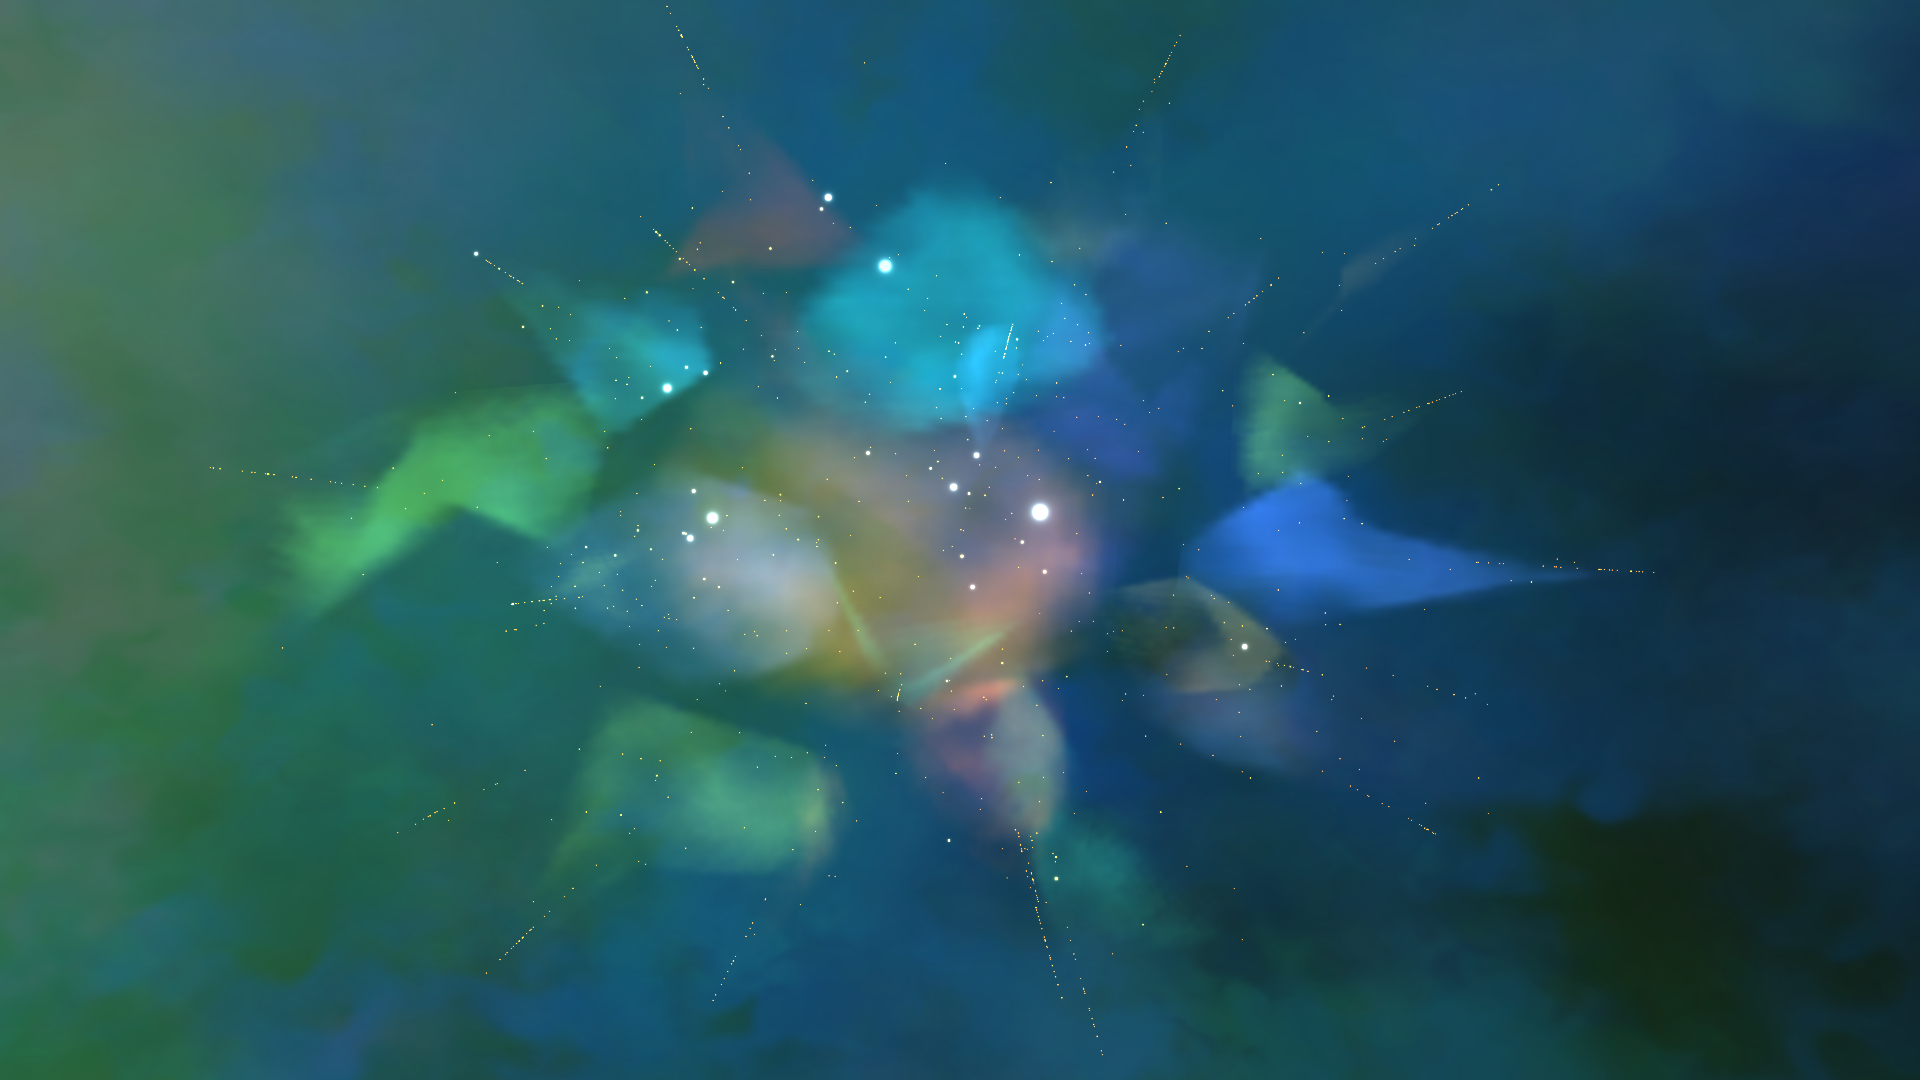
\includegraphics[width=1.0\linewidth, trim=32 160 32 160, clip]{graphics/softwaregalaxy-original.png}};
        \spy [cyan] on ($(arrows0.center)+(-2.3, +0.00)$) in node at ($(-6.8, -1.5)+(arrows0.center)$);
        \spy [magenta] on ($(arrows0.center)+(+2.3, -1.00)$) in node at ($(+6.8, +1.5)+(arrows0.center)$);
    \end{tikzpicture}
    \caption{%
        Nebula metaphor applied to the \emph{Software Galaxy}: 
        The left box highlights how documents are displayed as stars of varying intensities, the right box highlights how clusters of documents are visually grouped, using enclosing volumetric fog.}
   \label{Nebula}
 \end{teaserfigure}

\maketitle

\section{Introduction}

Software metrics provide a possibility for monitoring large software systems through mining software repositories and measuring aspects of complexity and quality of single source code files.
This can be useful for managing maintenance tasks.
As this is still a human task, software visualization is used to depict the state or the evolution of software through mapping metrics to the visual variables of 2D, 2.5D, or 3D viusalization techniques, e.g., Software Cities~\cite{steinbruckner2013-evolution}, or Gource~\cite{caudwell2010-gource}.
The layout of such a visualization technique is determined by the hierarchical structure of a project, which is helpful for navigating through a system.
However in many program comprehension tasks the question of detecting files that implement a similar concept arises. 
This motivates other approaches, which try to place the points based on their semantic relatedness~\cite{skupin2004worldofgeography, kuhn2008consistentlayout,achssld2021-softwareforest}.
\par
This work extends the approach for 2D \enquote{semantic layouts} to the third spatial dimension.
Our use of visual variables is inspired from the astronomical metaphor proposed by Lanza~\cite{lanza2001evolutionmatrix}, i.e., we display each file as a star with their own visual variables in space, thus resulting in a galaxy.
We further extend the metaphor by depicting clusters through volumetric nebulae.
Summarizing, this paper contributes a novel approach to depict software coding activities in a 3D virtual environment with star depictions and superimposed star clusters using a 3D layout based on semantic similarity.

\section{Software Galaxy Metaphor}

We extract the similarity directly from the source code.
Through the choice of identifier names and additional comments, developers encode semantics and domain knowledge directly in the source code, which can therefore be seen as a medium of communication between developers.
This motivates the use of text clustering techniques from the Natural Language Processing (NLP) domain to source code.
One of the most widely used class of NLP-techniques for clustering source code are Topic Models~\cite{chen2016survey}.
After applying various preprocessing steps to the vocabulary of the source code files, i.e., (1) stopword removal, (2) removal of keywords of the programming language, (3) identifier splitting, and (4) lemmatization, each document is stored as a Bag-of-Words vector thus neglecting the ordering of the words.
Latent Dirichlet Allocation (LDA) applied on the documents leads to a description of each document as a distribution over topics, which are in turn distributions over the vocabulary~\cite{blei2003latent}.
Measuring the distance between topics via the Jensen-Shannon distance, we project the topic-word-vectors onto the three-dimensional space using Multidimensional Scaling~\cite{cox2008multidimensional}.
The locations of the documents are determined by a linear combination of the topic vectors according to their document-topic-distribution~\cite{achssld2021-softwareforest}.

As visual mapping, we construct a 3D virtual scene where each document is located at its position in the layout.
In order to create stylistic stars, we apply point spread functions (PSF), in particular approximations of the Airy function.
We use the two basic attributes size and color as independent visual variables of the stars.
The size is used as input for the PSF and determines its radius.
A mapping that has shown its usefulness in our experiments was a mapping of the Lines-of-Code to size and the number of authors modifying a single file over time to color thus displaying the coding activities~\cite{knoeschke2020-thesis}.

With appropriate application of LDA and a dimension reduction, the proximity of points reflects their semantic similarity.
We emphasize this similarity by adding a cluster visualization that visually groups documents that implement a common semantic.
These clusters are depicted as semi-transparent volumes using a nebula metaphor.
The volume of a nebula is derived by alpha shapes applied to the cluster points and rendered by ray-tracing a low resolution 3D texture (one per nebula).
The nebula color is an additional visual variable that can depict the star density within a cluster.

Our prototype is an extension to a web-based, interactive 3D scatterplot framework implemented webgl-operate, WebGL, and TypeScript~\cite{wagner2020-scatterplot}. %
The point rendering is adapted to use PSFs and a volume rendering was added as well.
The available point labeling and interaction techniques are provided by the framework.

\section{Conclusions}
We proposed a 3D software visualization approach based on a layout representing the semantic structure and a galaxy metaphor for displaying the dynamic of the development process.
We plan to evaluate more topic modeling and dimension reduction techniques on various datasets of different size to find a best practice for generating semantic layouts~\cite{vernier2021-guided}.
Another step is to expand the idea of the star metaphor and improve the existing rendering quality.

\section*{Acknowledgements}
This work is part of the \enquote{Software-DNA} project, which is funded by the European Regional Development Fund (ERDF or EFRE in German) and the State of Brandenburg (ILB).
This work is part of the KMU project \enquote{KnowhowAnalyzer} (Förderkennzeichen 01IS20088B), which is funded by the German Ministry for Education and Research (Bundesministerium für Bildung und Forschung).

    \label{fig:basic-trans-vars}

\nocite{knoeschke2020-thesis}

\bibliographystyle{ACM-Reference-Format}
\bibliography{references}

\end{document}
\endinput
